\section{Probabilistic catalogs based on the 3FGL and 4FGL catalogs}
\lb{sec:prob_cats}

In this section we use the ML algorithms optimized in the previous section to construct probabilistic
classification of sources in the 3FGL and 4FGL catalogs.
%Having optimized our algorithms, we decided to test them on 3FGL data which was initially unassociated but then became associated in 4FGL. Furthermore, we tested the algorithms on 4FGL associated data, and also predicted for unassociated data.


\subsection{Probabilistic classification of sources in 3FGL and comparison with 4FGL}
\lb{sec:3FGLprediction1}


%In this section we perform probabilistic classification of sources in the 3FGL catalog.
We use the following four algorithms for the classification of sources: RF with 50 trees and maximal depth of 6, BDT with 100 trees and maximal depth of 2, NN with 11 neurons, LBFGS solver, and 300 epochs, and LR with LBFGS solver and 200 iterations. 
For training we use the pulsars and AGNs from the 3FGL catalog. In addition to original datasets, we perform oversampling of pulsars in order to balance the numbers of pulsars and AGNs.
As a result, we have 8 classification methods: 4 algorithms trained with and without oversampling.


\begin{table}[!h]
\hspace{-0.2cm}
\resizebox{0.47\textwidth}{!}{
    \tiny
  \centering
    \renewcommand{\tabcolsep}{0.4mm}
\renewcommand{\arraystretch}{1.6}

%\hspace{-3mm}
    \begin{tabular}{|c|c|c|c|c|c|c|}
    \hline
    Algorithm&Parameters &  Testing&Std. Dev.& Comparison with 4FGL \\
    & & Accuracy & & Accuracy \\
    \hline
    RF & 50 trees, max depth 6  &97.37&0.60& 91.41  \\
    RF\_O &   &97.90&0.50& 90.28 \\
    \hline %\midrule   -> aakash do you mean this?
    BDT & 100 trees, max depth 2    &   97.65&0.54&90.64 \\
%    \hline %\midrule   -> aakash do you mean this?
%    BDT & 200 trees, max depth 2    &   95.8  \\
    BDT\_O &     &   97.79&0.51& 90.79 \\
    \hline
    NN & 300 epochs, 11 neurons, LBFGS & 97.29&0.97& 89.32\\
    NN\_O &  & 94.31&5.13& 85.99\\
    \hline
    LR & 200 iterations, LBFGS solver & 97.63&0.54& 89.97 \\
    LR\_O &  &93.68&0.99& 85.55\\
    \hline
     
    \end{tabular}}
    \vspace{2mm}
    \caption{Testing accuracy of the 4 selected algorithms for classification of 3FGL sources and comparison with associations in the 4FGL-DR2 catalog. 
    ``\_O'' denotes training with oversampling.}
    \label{tab:selected_algs}
\end{table}



\begin{figure*}[h]
\centering
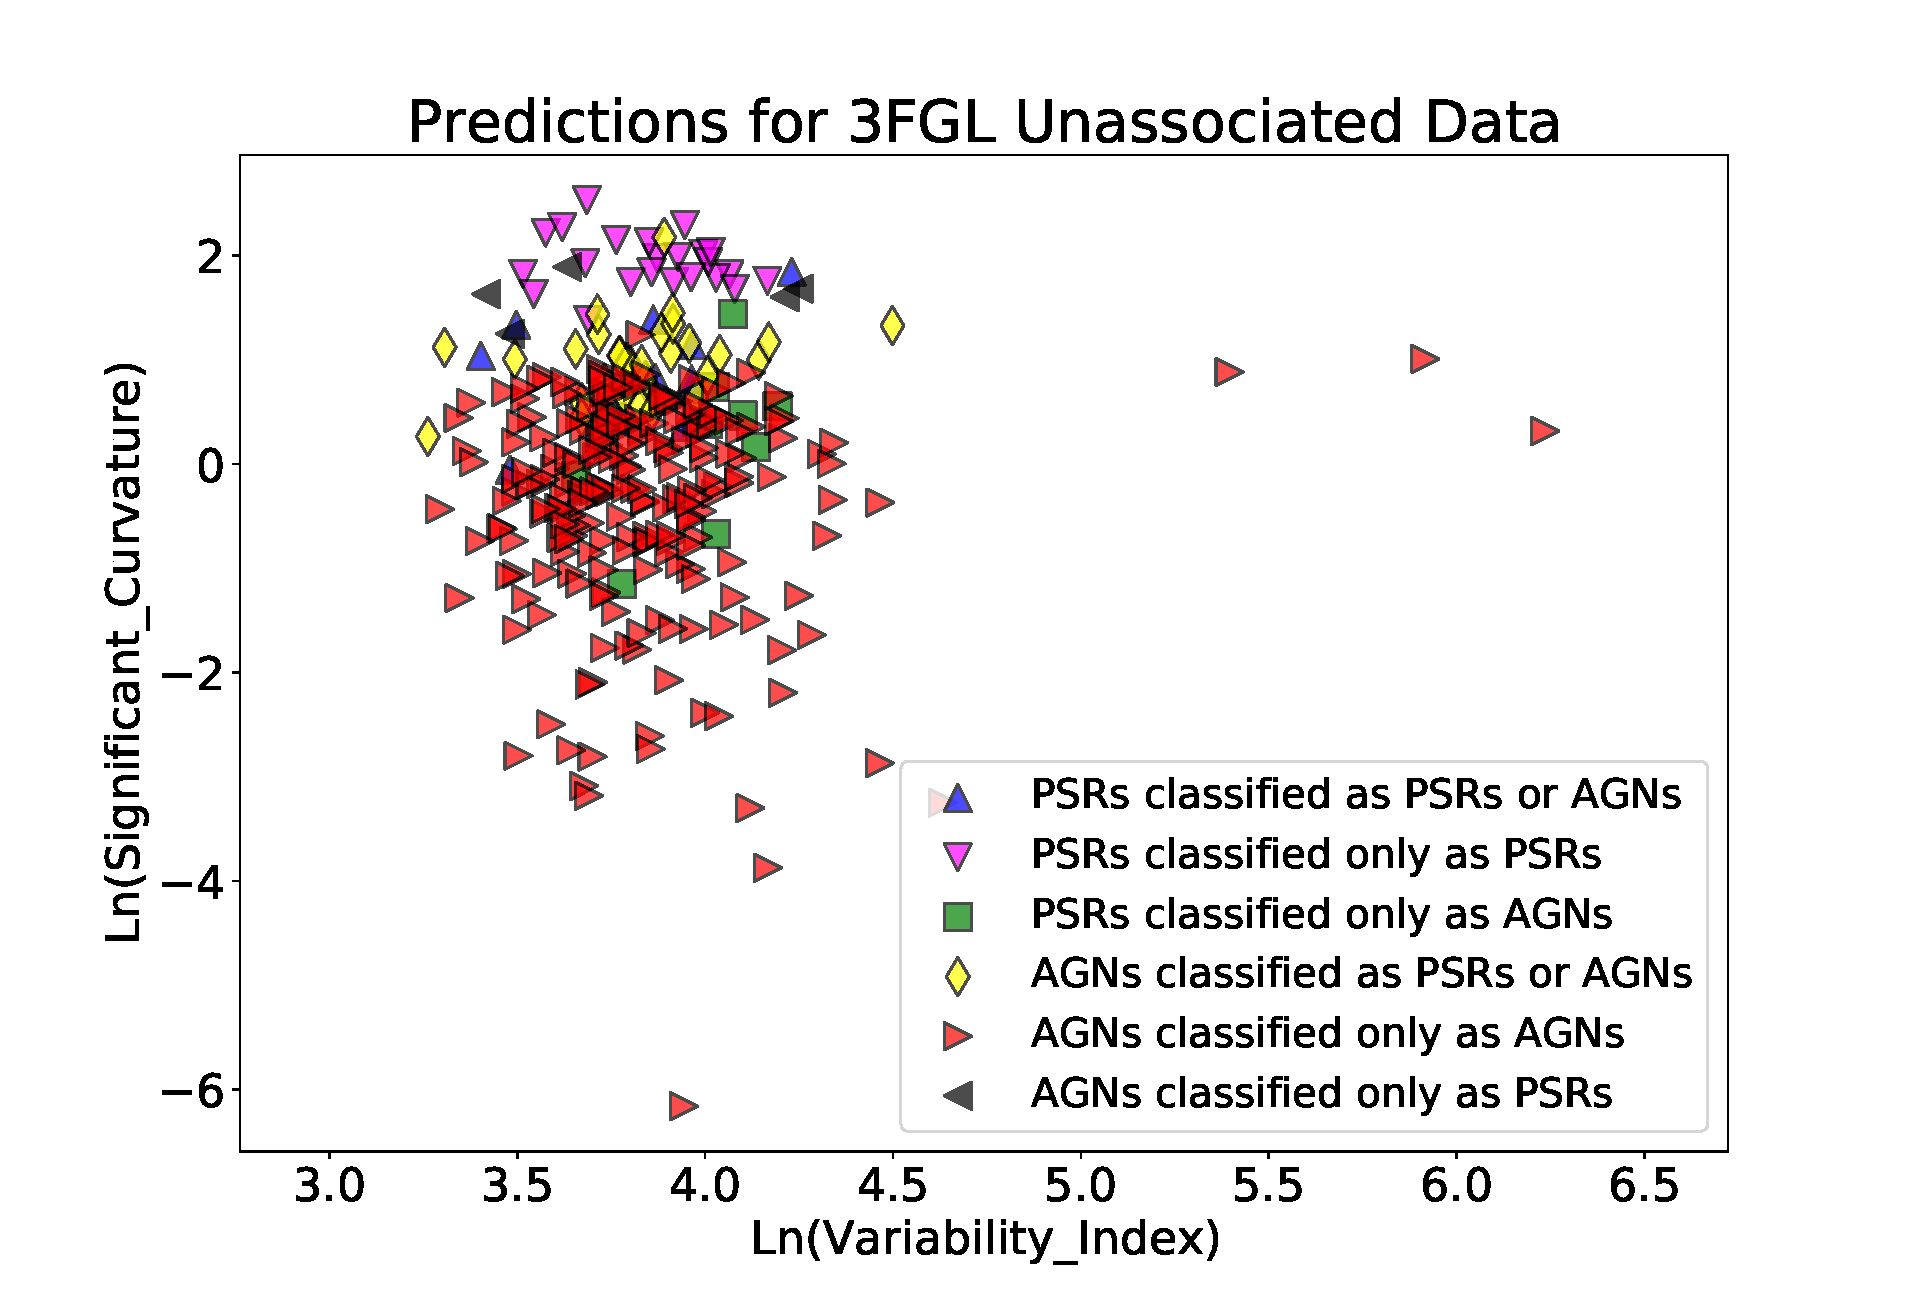
\includegraphics[width=0.8\textwidth]{plots/plot_final_DR2.pdf}
%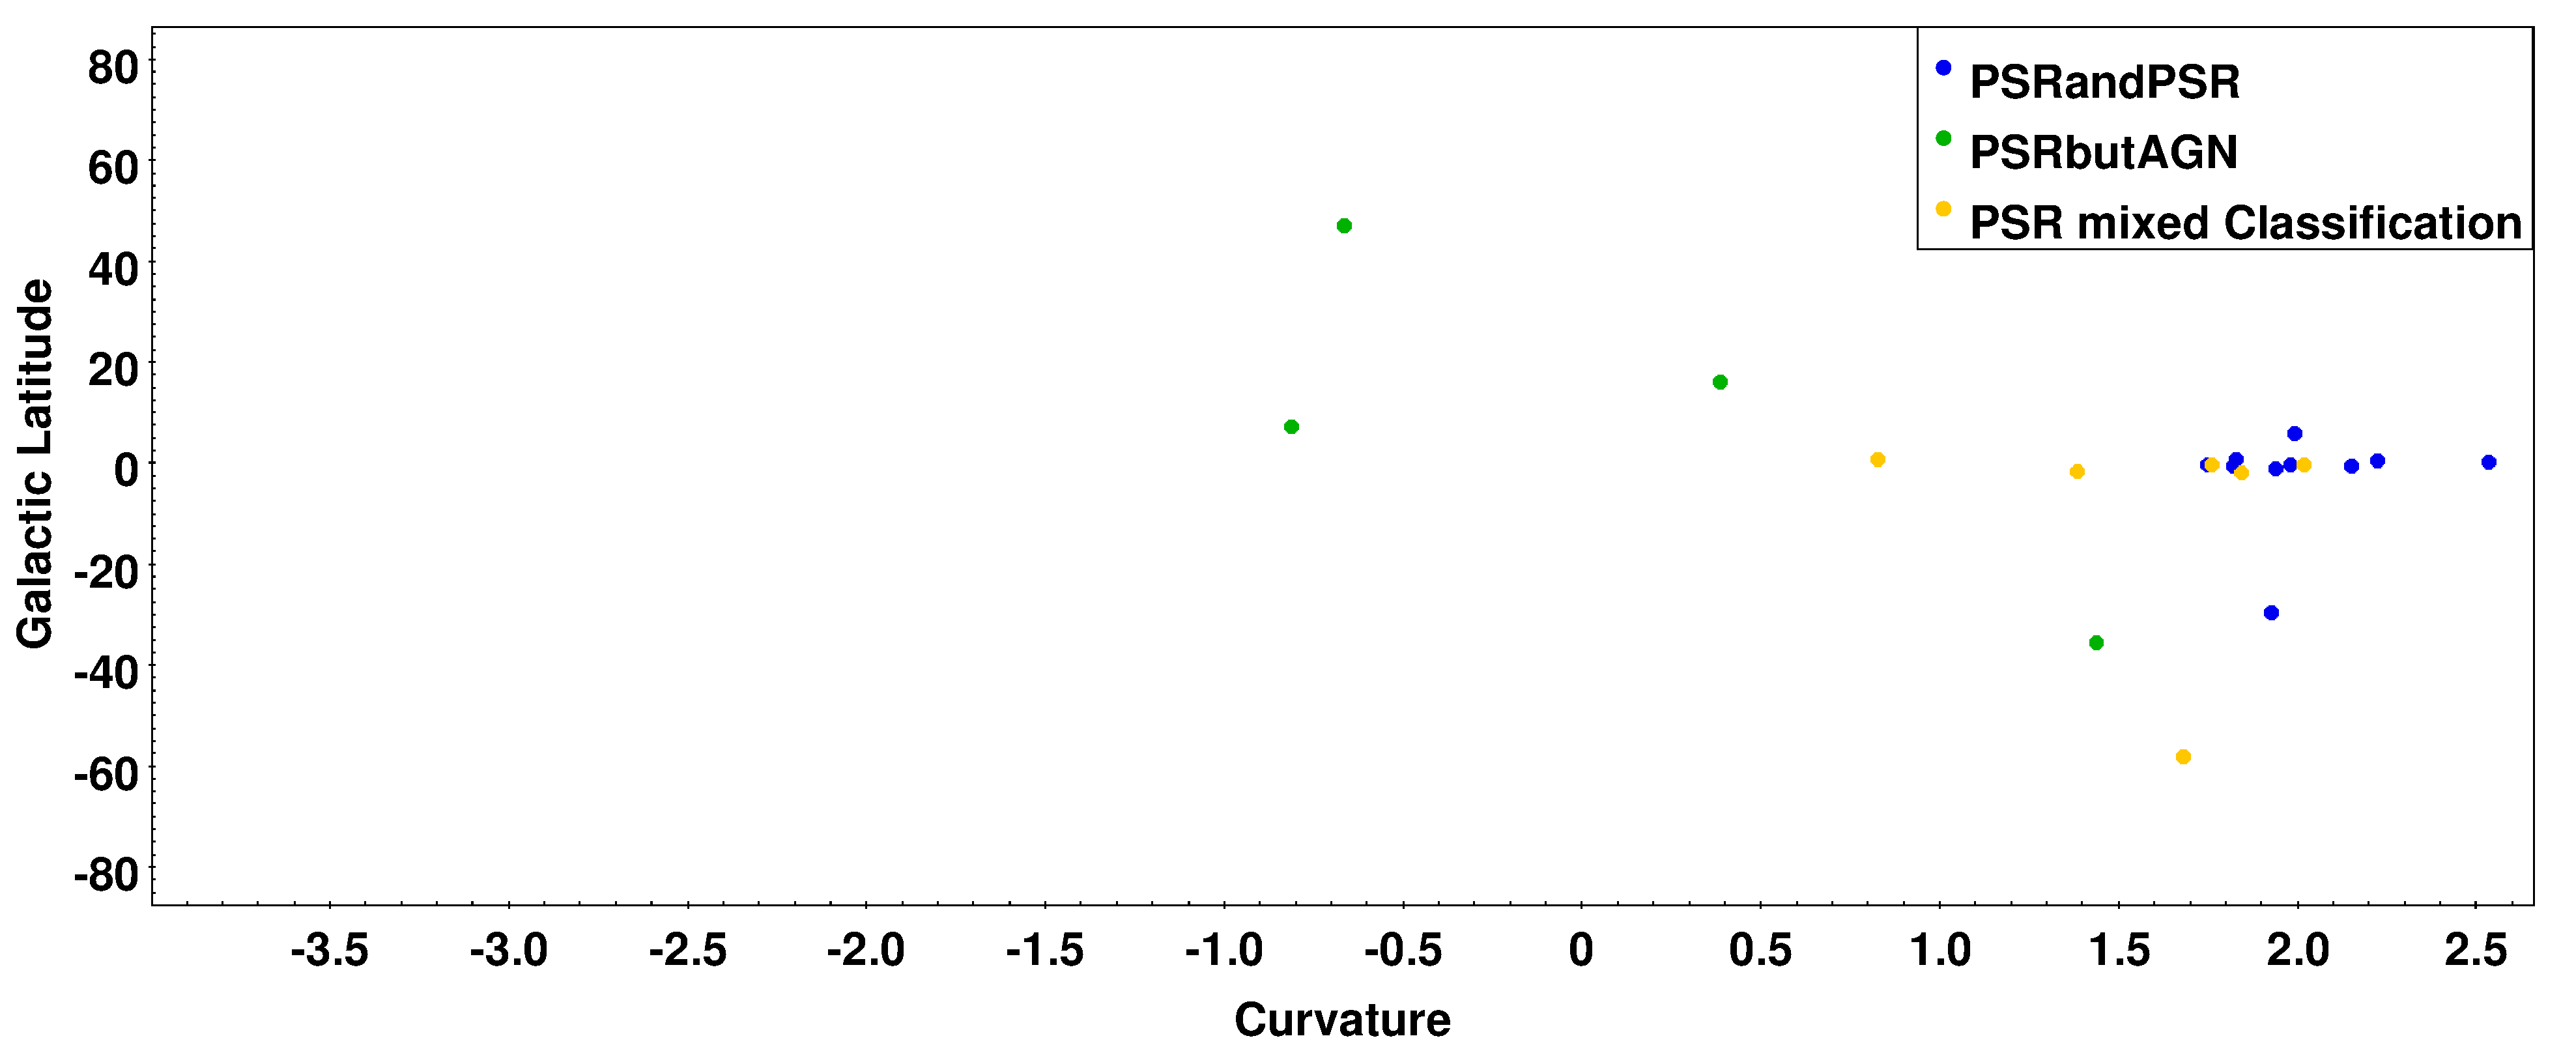
\includegraphics[width=\twopicsp\textwidth]{plots/PSR3.pdf}
\caption{Comparison of class prediction for unassociated 3FGL sources with classes in 4FGL DR2. 
For more details see Section \ref{sec:3FGLprediction1}.}
%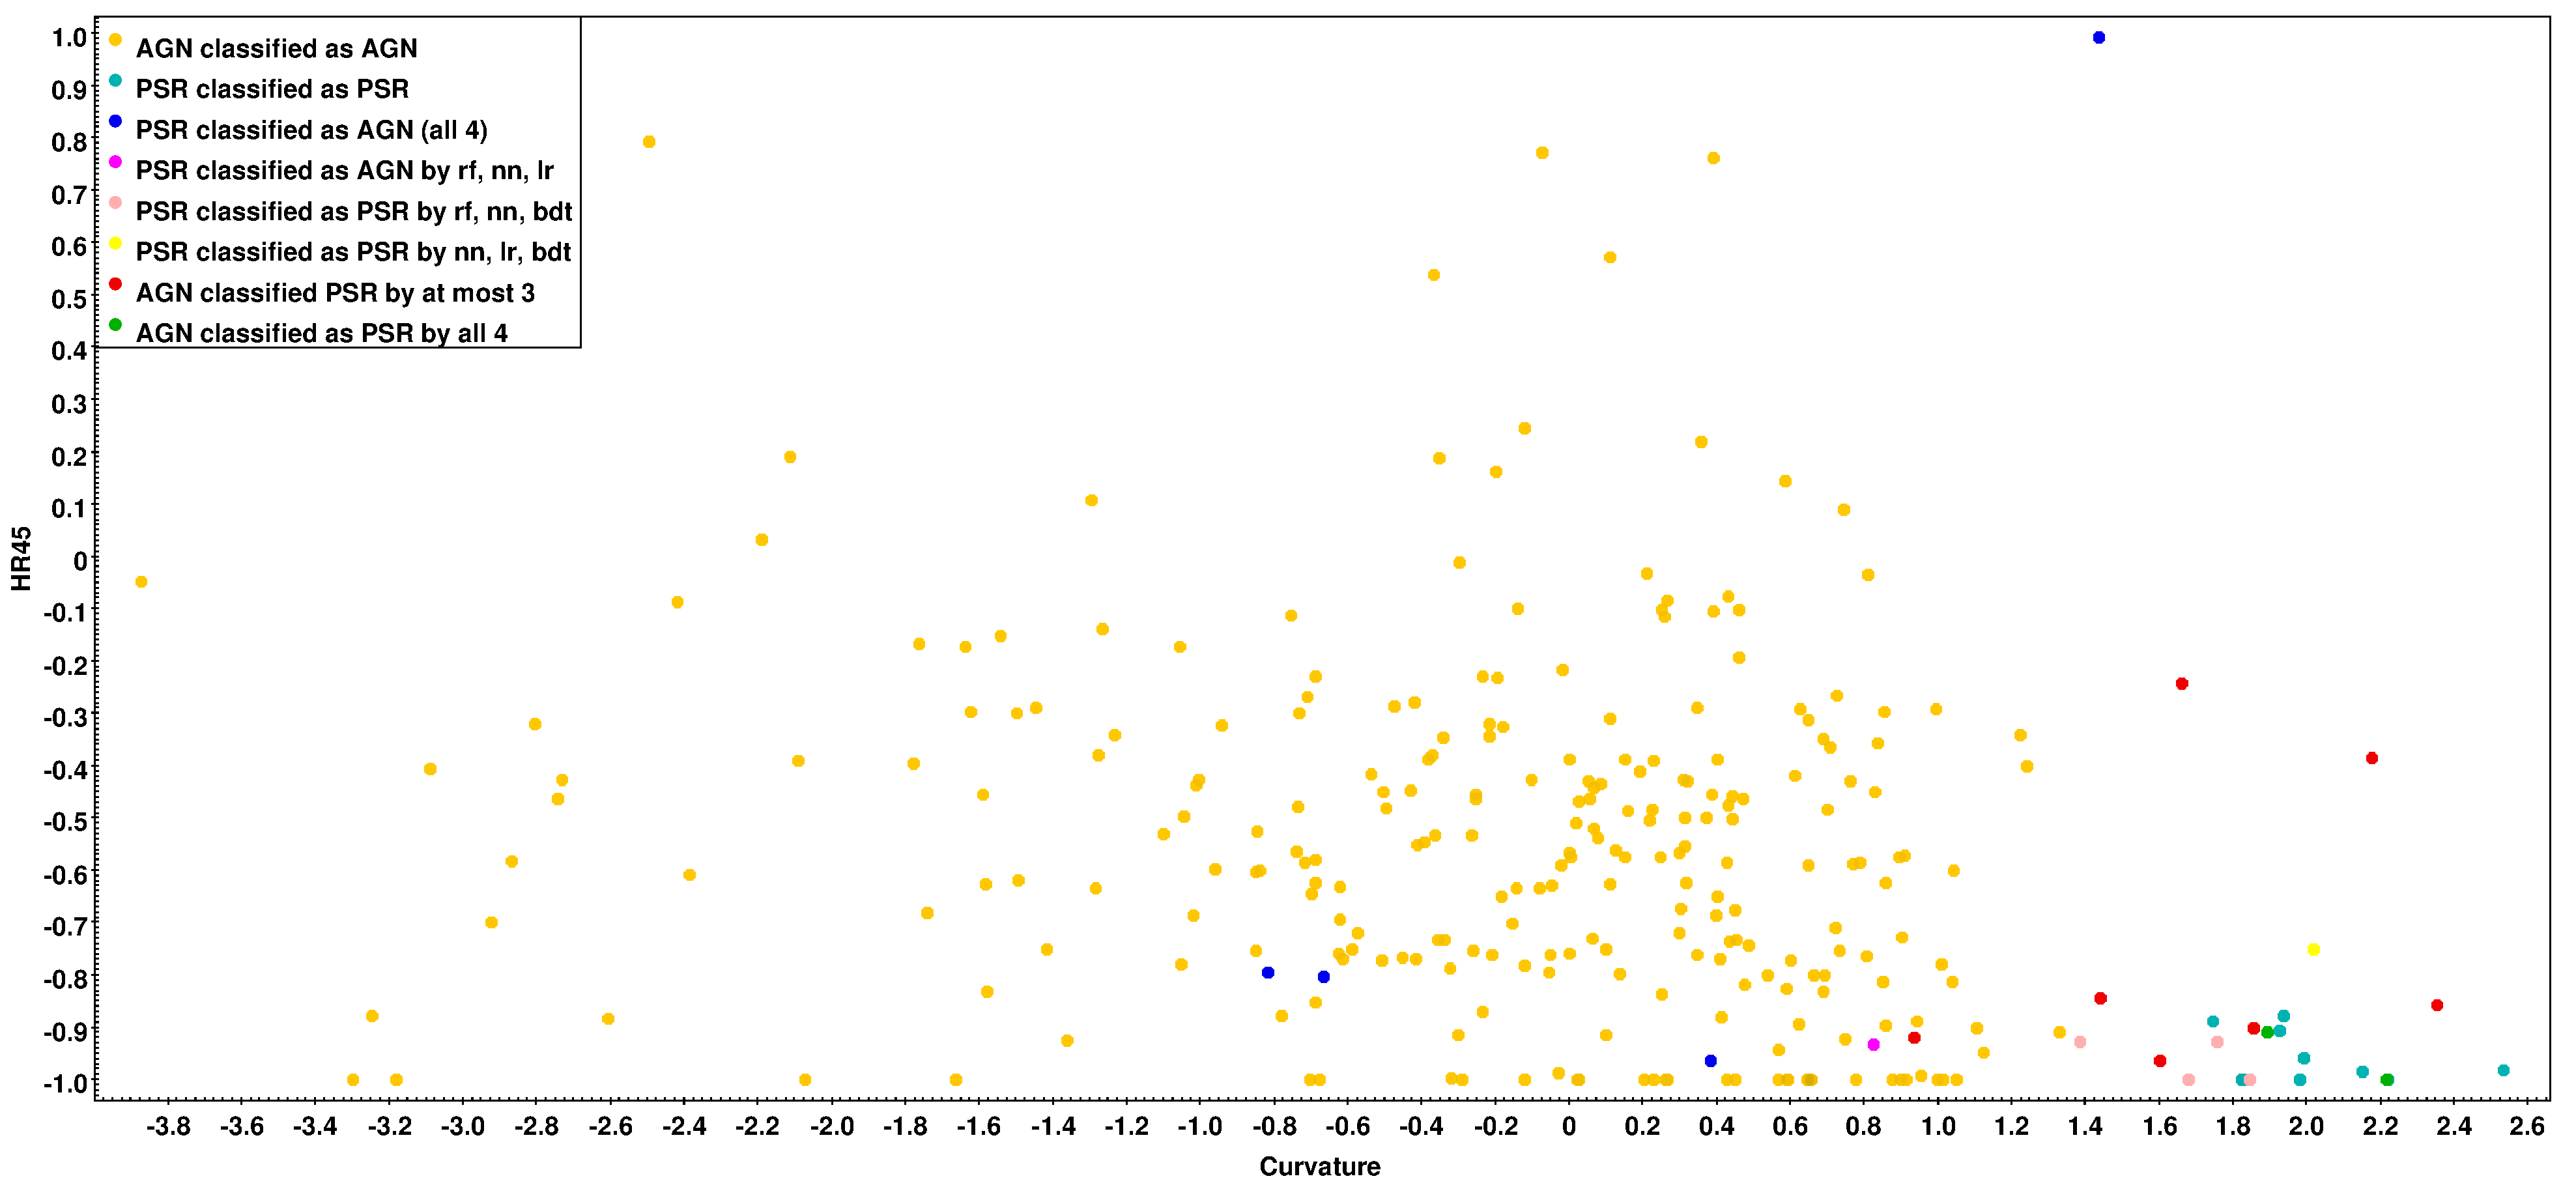
\includegraphics[width=\twopicsp\textwidth]{plots/final_catalog.pdf}
\label{fig:3FGL_vs_4FGL_classes}
\end{figure*}

The selected algorithms are summarized in Table \ref{tab:selected_algs}, where oversampling is shown by ``\_O''.
``Average testing accuracy'' is computed by taking 1000 times 70\% - 30\% split into training and testing samples and averaging over the 
accuracies computed for the testing samples.
In addition, we look at sources, which are unassociated in 3FGL but have either pulsar or AGN association in 4FGL: there are 278 such sources.
The accuracy of our prediction for the four selected algorithms with and without oversampling, taking the 4FGL classes as the true values, is reported in the column ``Comparison with 4FGL Accuracy''.
The correct classifications and misclassifications for the 278 sources with associations in 4FGL are also presented in Figure \ref{fig:3FGL_vs_4FGL_classes}.
The class at the beginning of the label name corresponds to the association in the 4FGL, while the second half of the labels corresponds to classification of unassociated sources in 3FGL. For example, ``PSRs classified only as PSRs'' shows sources which have PSR association in 4FGL and all eight methods classified the corresponding unassociated sources in 3FGL as a pulsar. ``PSRs classified as either PSRs or AGNs'' labels sources with PSR associations in 4FGL but the corresponding unassociated sources in 3FGL have both PSR and AGN classifications by different ML methods.
The unassociated sources are classified as PSRs or AGNs if the corresponding probability is larger than 0.5.
We notice that misclassified or partially misclassified sources in Figure \ref{fig:3FGL_vs_4FGL_classes} typically happen on the boundary between the two classes or even inside the opposite class.
Many of these sources also have flags in the 3FGL catalog, such as a potential problem with the background diffuse emission model in the location of the source, which can lead to a poor reconstruction of the source spectrum and, consequently, misclassification of the source.


As a result of the classification with the eight ML methods,
we created a probabilistic catalog based on the 3FGL sources without missing values.%
\footnote{There are thirteen sources with missing values in the 3FGL catalog (2 unassociated, 5 AGNs, 1 pulsar, and 5 ``other'' sources), 
which we save in a separate file ``3FGL\_sources\_with\_missing\_values.csv'' for reference.}
We train on 70\% of the sources associated with pulsars or AGNs and save the probability values for testing sources, for sources which are not classified as pulsars or AGNs, and for unassociated sources.
We repeat the splitting and training 1000 times and report the sample average and standard deviation of the classification probabilities,
i.e., we average over 1000 values for unassociated sources and sources not classified as AGNs or pulsars, 
while the average for AGNs and pulsar is over the number of times the sources appear in the testing sample, which is 300 on average.
%Like in the case of associated sources, where we split the data 1000 times, we also do a 1000 runs for the unassociated case. This allows us to calculate individual probabilities and their standard deviations for all sources.
%\dima{Classification of associated sources is done by averaging over testing-training samples splits.
%Do we also do averaging for unassociated sources?}

We have also subselected the 278 unassociated 3FGL sources, which have PSR or AGN associations in 4FGL,
and saved them for convenience of comparison as a separate file.
In the probabilistic catalogs we add columns with corresponding probabilities for each algorithm and each class,
i.e., provided that there are 8 methods (including oversampling) and 2 classes, we add 16 columns: 8 for unweighted and 8 for oversampled training data. The columns with '\_O' represent the oversampled probabilities. We also add 16 columns for standard deviations of probabilities. Although class probabilities and standard deviation for each algorithm are not independent (probabilities add up to 1 and standard deviations are equal for AGN and PSR classes), we keep the corresponding columns in view of possible generalizations to multi-class classification.
%Although the class probabilities for each algorithms should add up to one for every source, we still keep the columns for all classes for convenience.
Table \ref{tab:prob_cat} shows an example of the probabilistic catalog for a few unassociated 3FGL sources.
Notice that the first source is classified as a pulsar by BDT and as an AGN by RF, LR, and NN algorithms,
it is an example of a source with mixed classification.
%i.e., it has a label ``classified either as PSRs or AGNs'' in Figure \ref{fig:3FGL_vs_4FGL_classes}. - is it associated in 4FGL?
%The second and third sources are classified as AGNs by all four algorithms, i.e., they will have a label ``classified only as AGNs'',
%while the last source is classified as a pulsar by all four algorithms, i.e., it will have a label ``classified only as PSRs''.
Out of 1008 unassociated sources in 3FGL, 111 are classified as pulsars by all eight methods, 597 are classified as AGNs, and 300 have mixed classifications.
Out of 111 sources classified as pulsars, 6 sources have counterparts in Parkes survey \citep{Camilo2015} within 2 arc minutes (see Table \ref{tab:parkes}).

We summarize the results of classification of the unassociated 3FGL sources in Table \ref{tab:3FGL_prediction}.
The ``AGNs'' column shows the number of unassociated sources where all eight methods from Table \ref{tab:selected_algs} give the probability for a source to be an AGN above 50\%.
Similarly the ``Pulsars'' column shows the number of unassociated sources where all four algorithms predict the source to be more likely a pulsar.
The ``Mixed'' column shows the number of sources with mixed classification, i.e., some algorithms predict that the source is more likely an AGN while the other algorithms predict that it is more likely a pulsar.
In the ``Uncorrected'' row we do not take into account that there can be sources other than AGNs or pulsars among the unassociated sources.
We correct for the presence of the other sources by assuming that the fraction of AGN-like and pulsar-like sources among the other sources is the same for associated and for unassociated sources.
In particular, we denote by $N_{\rm AGN}$ the number of unassociated sources with AGN-like classification by all four algorithms,
by $N_{\rm AGN}^{\rm ass\,other}$ the number of sources with AGN-like classification among associated other sources,
by $N_{\rm ass}$ ($N_{\rm unass}$) the total number of associated (unassociated) sources.
The number of AGN-like sources among the unassociated source corrected for the presence of other sources is estimated as

\be
\lb{eq:other_correction}
N_{\rm AGN}^{\rm corr} = N_{\rm AGN} - N_{\rm AGN}^{\rm ass\,other} \,\frac{N_{\rm unass}}{N_{\rm ass}}.
\ee
Analogous corrections are applied for the number of unassociated sources with pulsar-like classification by all eight methods,
and for unassociated sources with mixed classification.




\pgfplotstableread[col sep=comma]{tables/3FGL_unassoc_vs_4FGL_assoc.csv}\loadedtable
\begin{table}
\pgfplotstabletypeset[columns={Source_Name_3FGL,AGN_BDT,AGN_RF,AGN_LR,AGN_NN},
column type=l,
string type,
every head row/.style={before row={\toprule & \multicolumn{4}{c}{AGN Probability} \\},after row=\midrule,},
every last row/.style={after row=\midrule}, %\vdots },
columns/Source_Name_3FGL/.style={column name=Source\_Name\_3FGL},
columns/AGN_BDT/.style={column name=BDT,numeric type,fixed,precision=3},
columns/AGN_NN/.style={column name=NN,numeric type,fixed,precision=3},
columns/AGN_RF/.style={column name=RF,numeric type,fixed,precision=3},
columns/AGN_LR/.style={column name=LR,numeric type,fixed,precision=3},
skip rows between index={4}{302}
]\loadedtable
\caption{\label{tab:prob_cat}
Example of the AGN classification probabilities for a few unassociated sources in the 3FGL catalog \citep{2015ApJS..218...23A}. We have ommited the oversampled probability columns here.}
\end{table}




\pgfplotstableread[col sep=comma]{tables/3fgl_unassoc_predictions_matches_with_Parkes(2015)_1.csv}\loadedtable
\begin{table}
\pgfplotstabletypeset[columns={Source_Name_3FGL,GLON,GLAT,Separation},
column type=l,
string type,
every head row/.style={before row={\toprule},after row=\midrule,},
every last row/.style={after row=\midrule },
columns/Source_Name_3FGL/.style={column name=Source\_Name\_3FGL},
columns/GLON/.style={column name=GLON,numeric type,fixed,precision=1},
columns/GLAT/.style={column name=GLAT,numeric type,fixed,precision=1},
columns/Separation/.style={column name=Sep (arksec),numeric type,fixed,precision=1}
]\loadedtable
\caption{\label{tab:parkes}
Connection of unassociated 3FGL sources classified as pulsars with Parkes pulsars \citep{Camilo2015}.}
\end{table}



\begin{table}[!h]
\resizebox{0.45\textwidth}{!}{
    \tiny
 %  \centering
    \renewcommand{\tabcolsep}{0.3mm}
\renewcommand{\arraystretch}{1.5}

    \begin{tabular}{| l |c|c|c|}
    \hline
    Correction for other sources & AGNs & Pulsars & Mixed \\
    \hline
    Uncorrected &  597 & 111  &  300 \\
    \hline
    Corrected & 578  & 97  & 279 \\
    \hline
     
    \end{tabular}}
    \vspace{0.2cm}
    \caption{Expected number of AGNs and pulsars among the unassociated 3FGL sources.
    ``AGNs'' and ``Pulsars'' columns show the number of sources where all eight methods predict the same class,
    ``Mixed'' column shows the number of sources with mixed classification.
    Uncorrected (corrected) rows show the number of predicted AGNs and pulsars among the unassociated sources, which are
    uncorrected (corrected) for the presence of sources other than AGNs and pulsars among the unassociated sources.}
    \label{tab:3FGL_prediction}
\end{table}



\subsection{Probabilistic classification of sources in the 4FGL-DR2 catalog}
\lb{sec:4FGLprediction}

In this section we construct a probabilistic classification of sources in the 4FGL-DR2 catalog. The 4FGL-DR2 catalog \citep{2020arXiv200511208B} 
is based on 10 years of \Fermi-LAT data \citep[compared to 8 years of data in the 4FGL catalog,][]{2020ApJS..247...33A}.
It contains 5788 sources, which is 723 sources more than in the 4FGL catalog (all sources in 4FGL are kept in 4FGL-DR2 even if they fall
below the detection threshold with 10 years of data). Out of these 3770 sources have either a classification of AGN or a PSR, 1658 are unassociated (we only look at CLASS1 column in the catalog), and the rest 346 sources are other sources with classification like PWN or SNR, etc.
There are 14 sources in 4FGL-DR2 with missing values: four AGNs, one PWN (Crab), and nine unassociated sources.
As in the previous section, we use for training and testing sources associated with either AGNs or pulsars,
which have no missing values used for classification.%
%\footnote{In the 4FGL catalog there is only one source with missing values: 4FGL J0534.5+2201i associated with the Crab pulsar wind nebula.}
We then calculate the classification probabilities of AGN and PSR classes for both the associated and the unassociated sources.
The 4FGL catalog has higher number of features, especially due to the difference in modeling of the spectra compared with the 3FGL catalog. 
We selected 28 of these features and looked for correlations among them. If any feature was correlated or anti-correlated with a Pearson index of $\pm$0.75 or higher with another feature, then only one of these features was kept. 
%The correlation matrix is shown in Figure \ref{fig:corr_mat}.
The resulting 16 features are:
GLON, GLAT, ln(Pivot\_Energy), ln(Energy\_Flux100),ln(Unc\_Energy\_Flux100), LP\_Index, Unc\_LP\_Index, LP\_beta, LP\_SigCurv, hr12, hr23, hr34, hr45, hr56, hr67, ln(Variability\_Index).
Some of these features are directly counterparts to the features which we used in the 3FGL catalog,
e.g., GLAT, LP\_Index (instead of Spectral\_Index or 500MeV\_Index), LP\_SigCurv (instead of ln(Signif\_Curve)), 
ln(Variability\_Index), hardness ratios (in the 4FGL catalog there are two more energy bins compared to the 3FGL catalog).

\begin{comment}
\begin{figure*}[h]
\centering
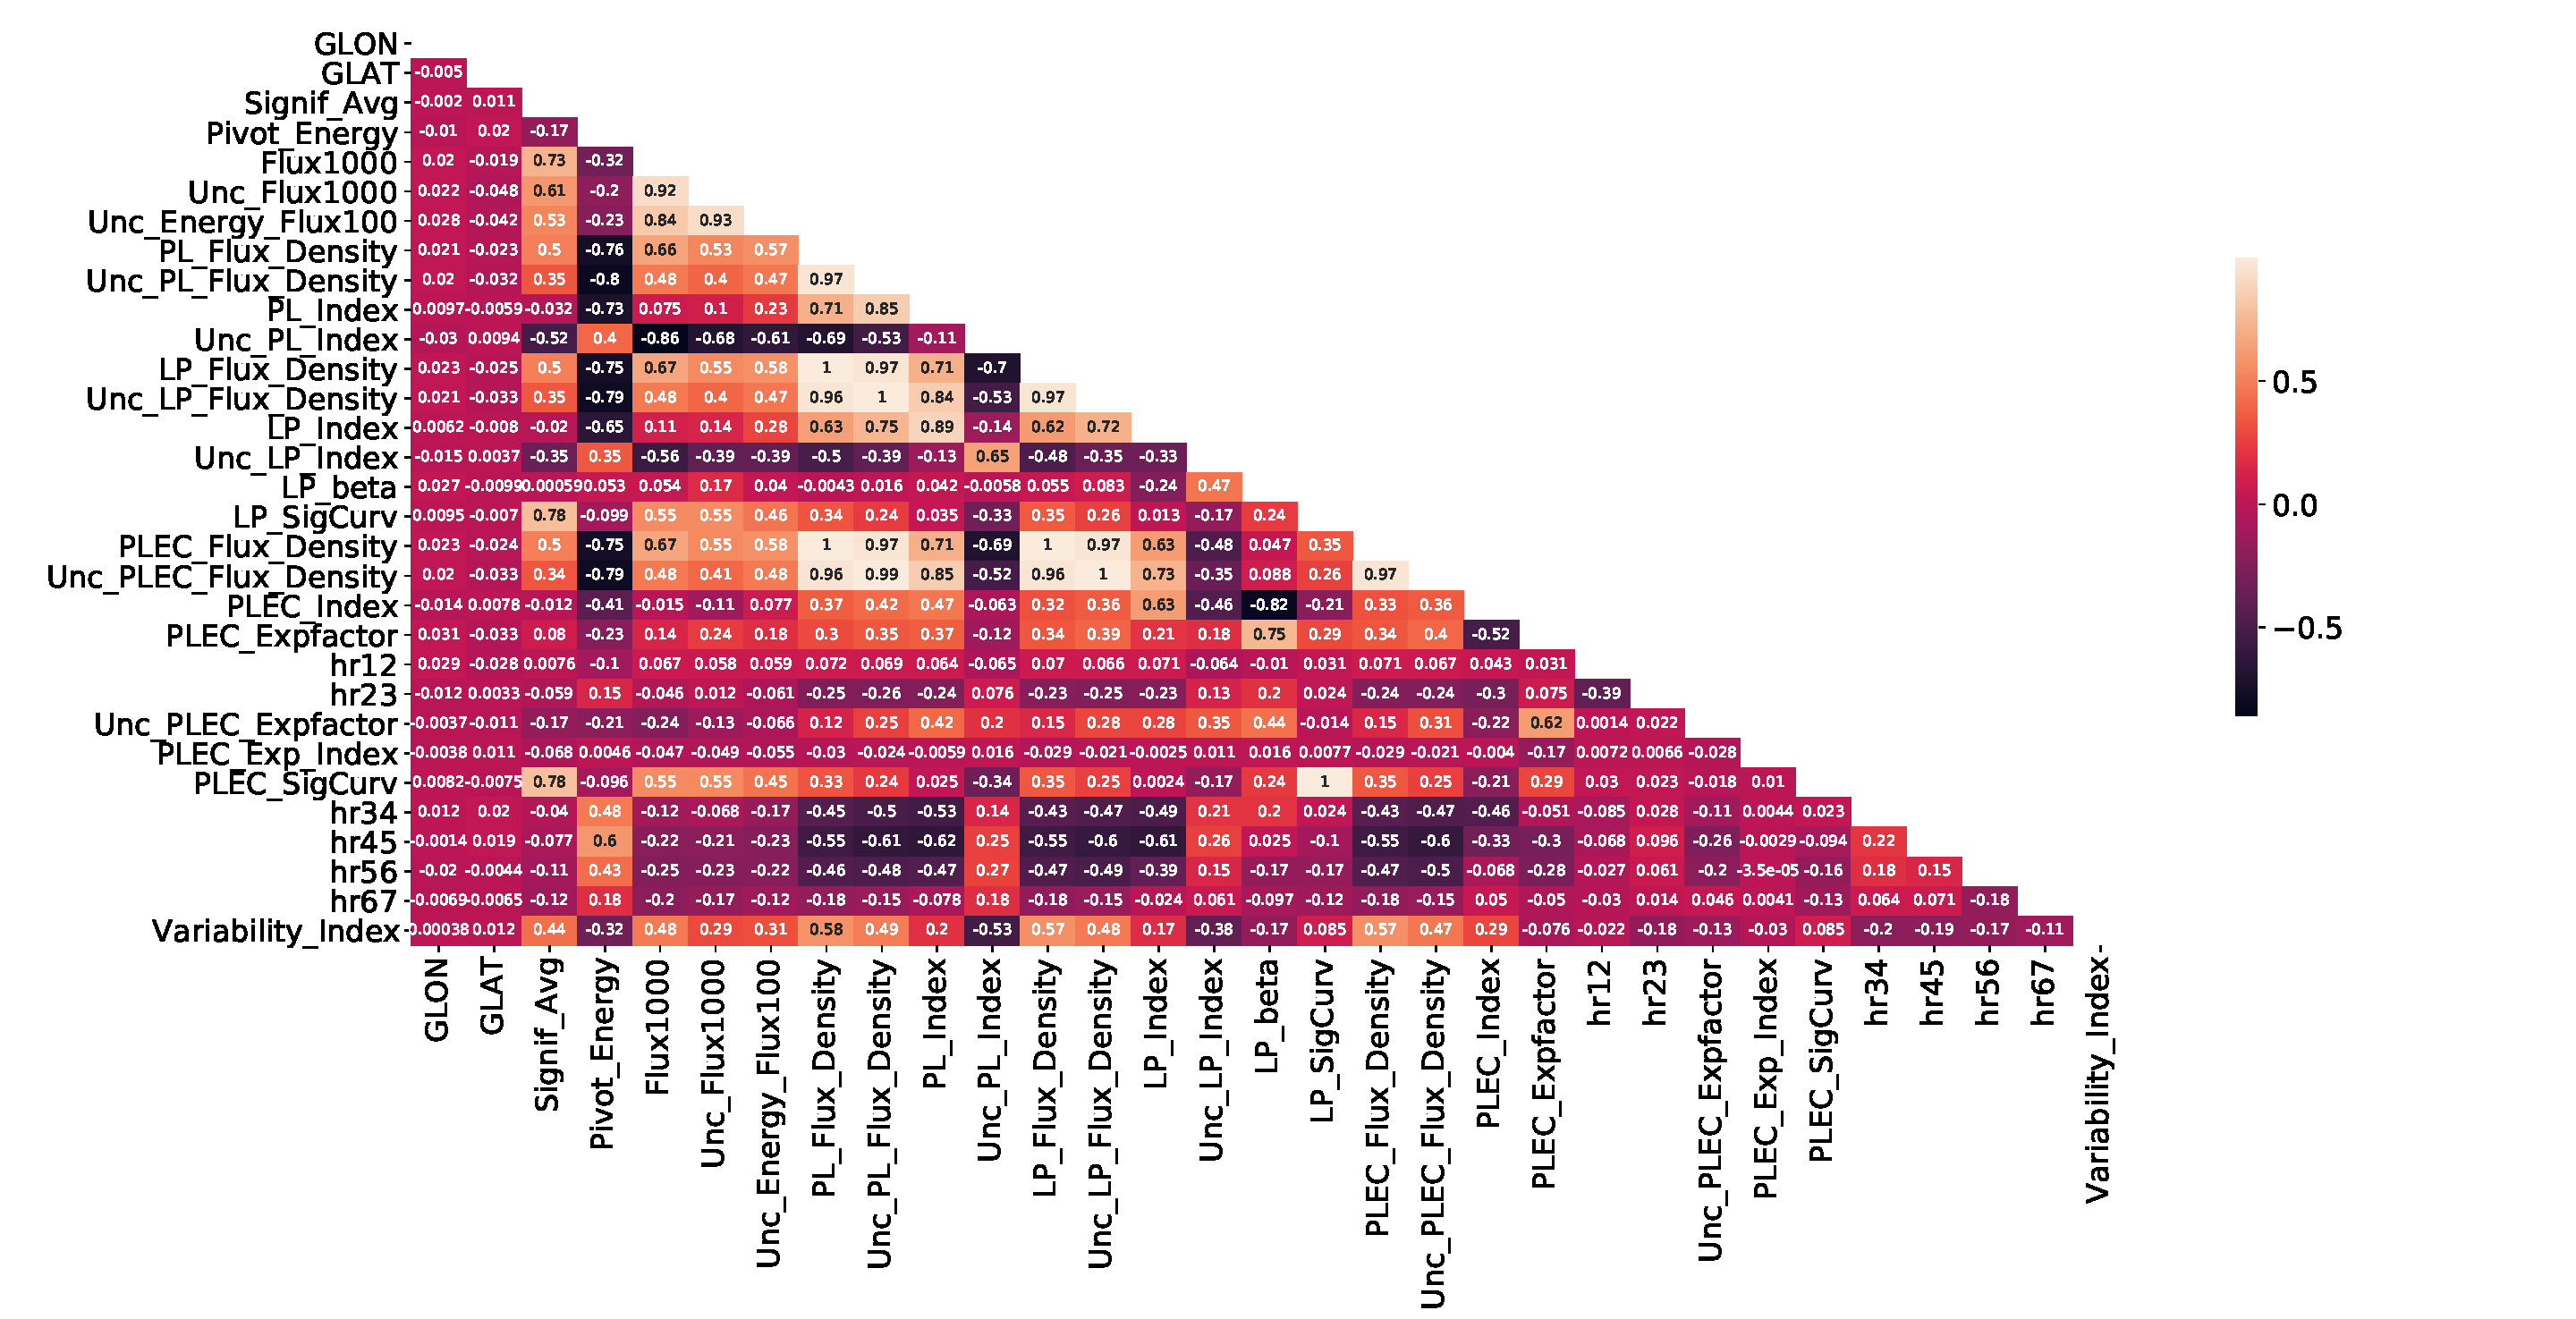
\includegraphics[width=\textwidth]{plots/correlation_4fgl_assoc.pdf}
%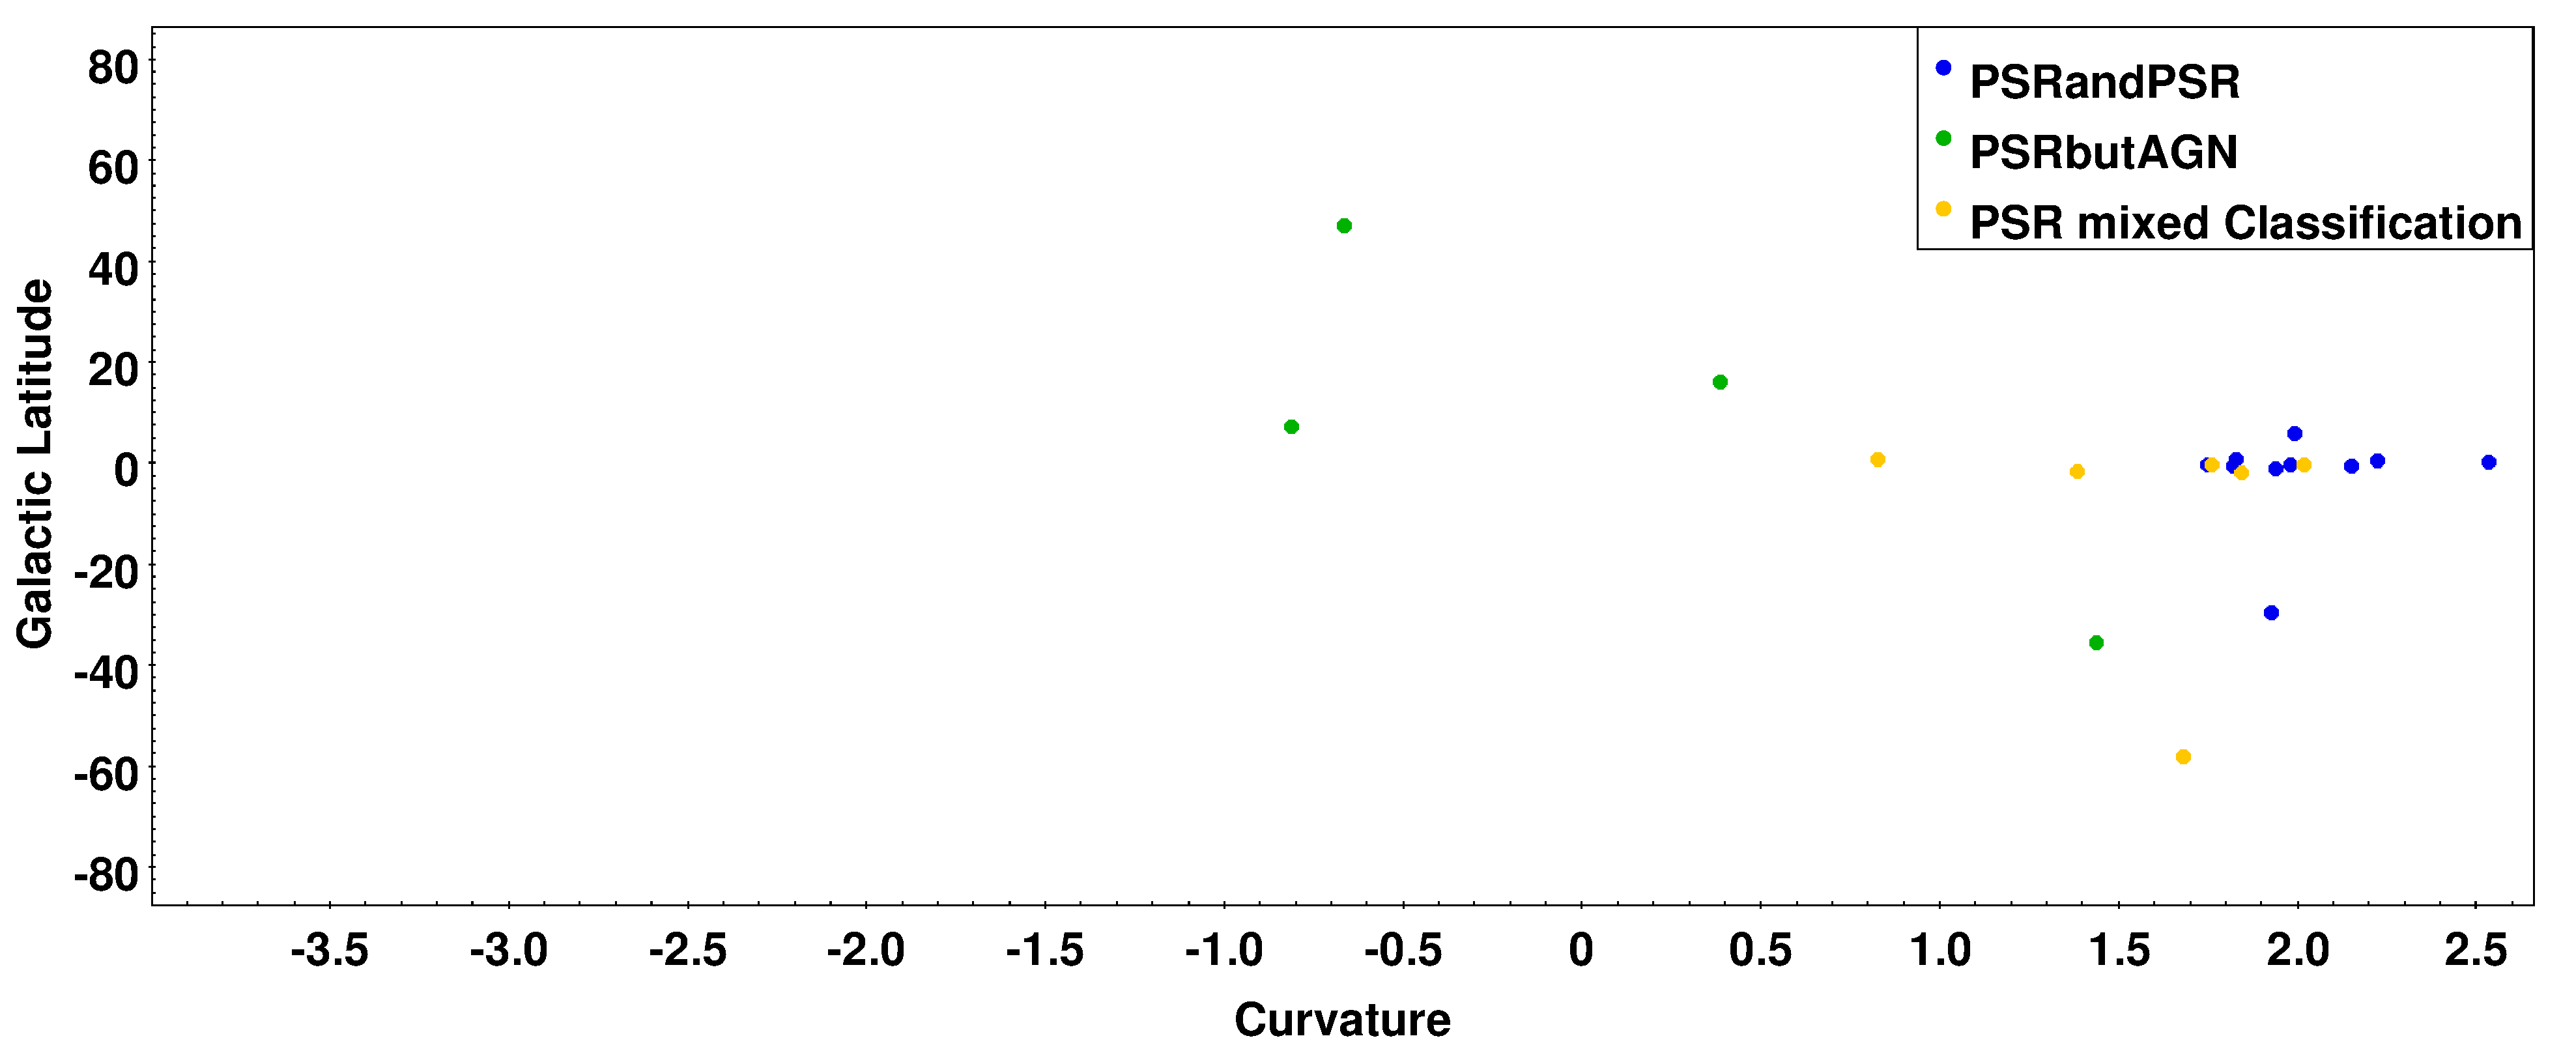
\includegraphics[width=\twopicsp\textwidth]{plots/PSR3.pdf}
\caption{Corelation matrix for 4FGL associated data }
%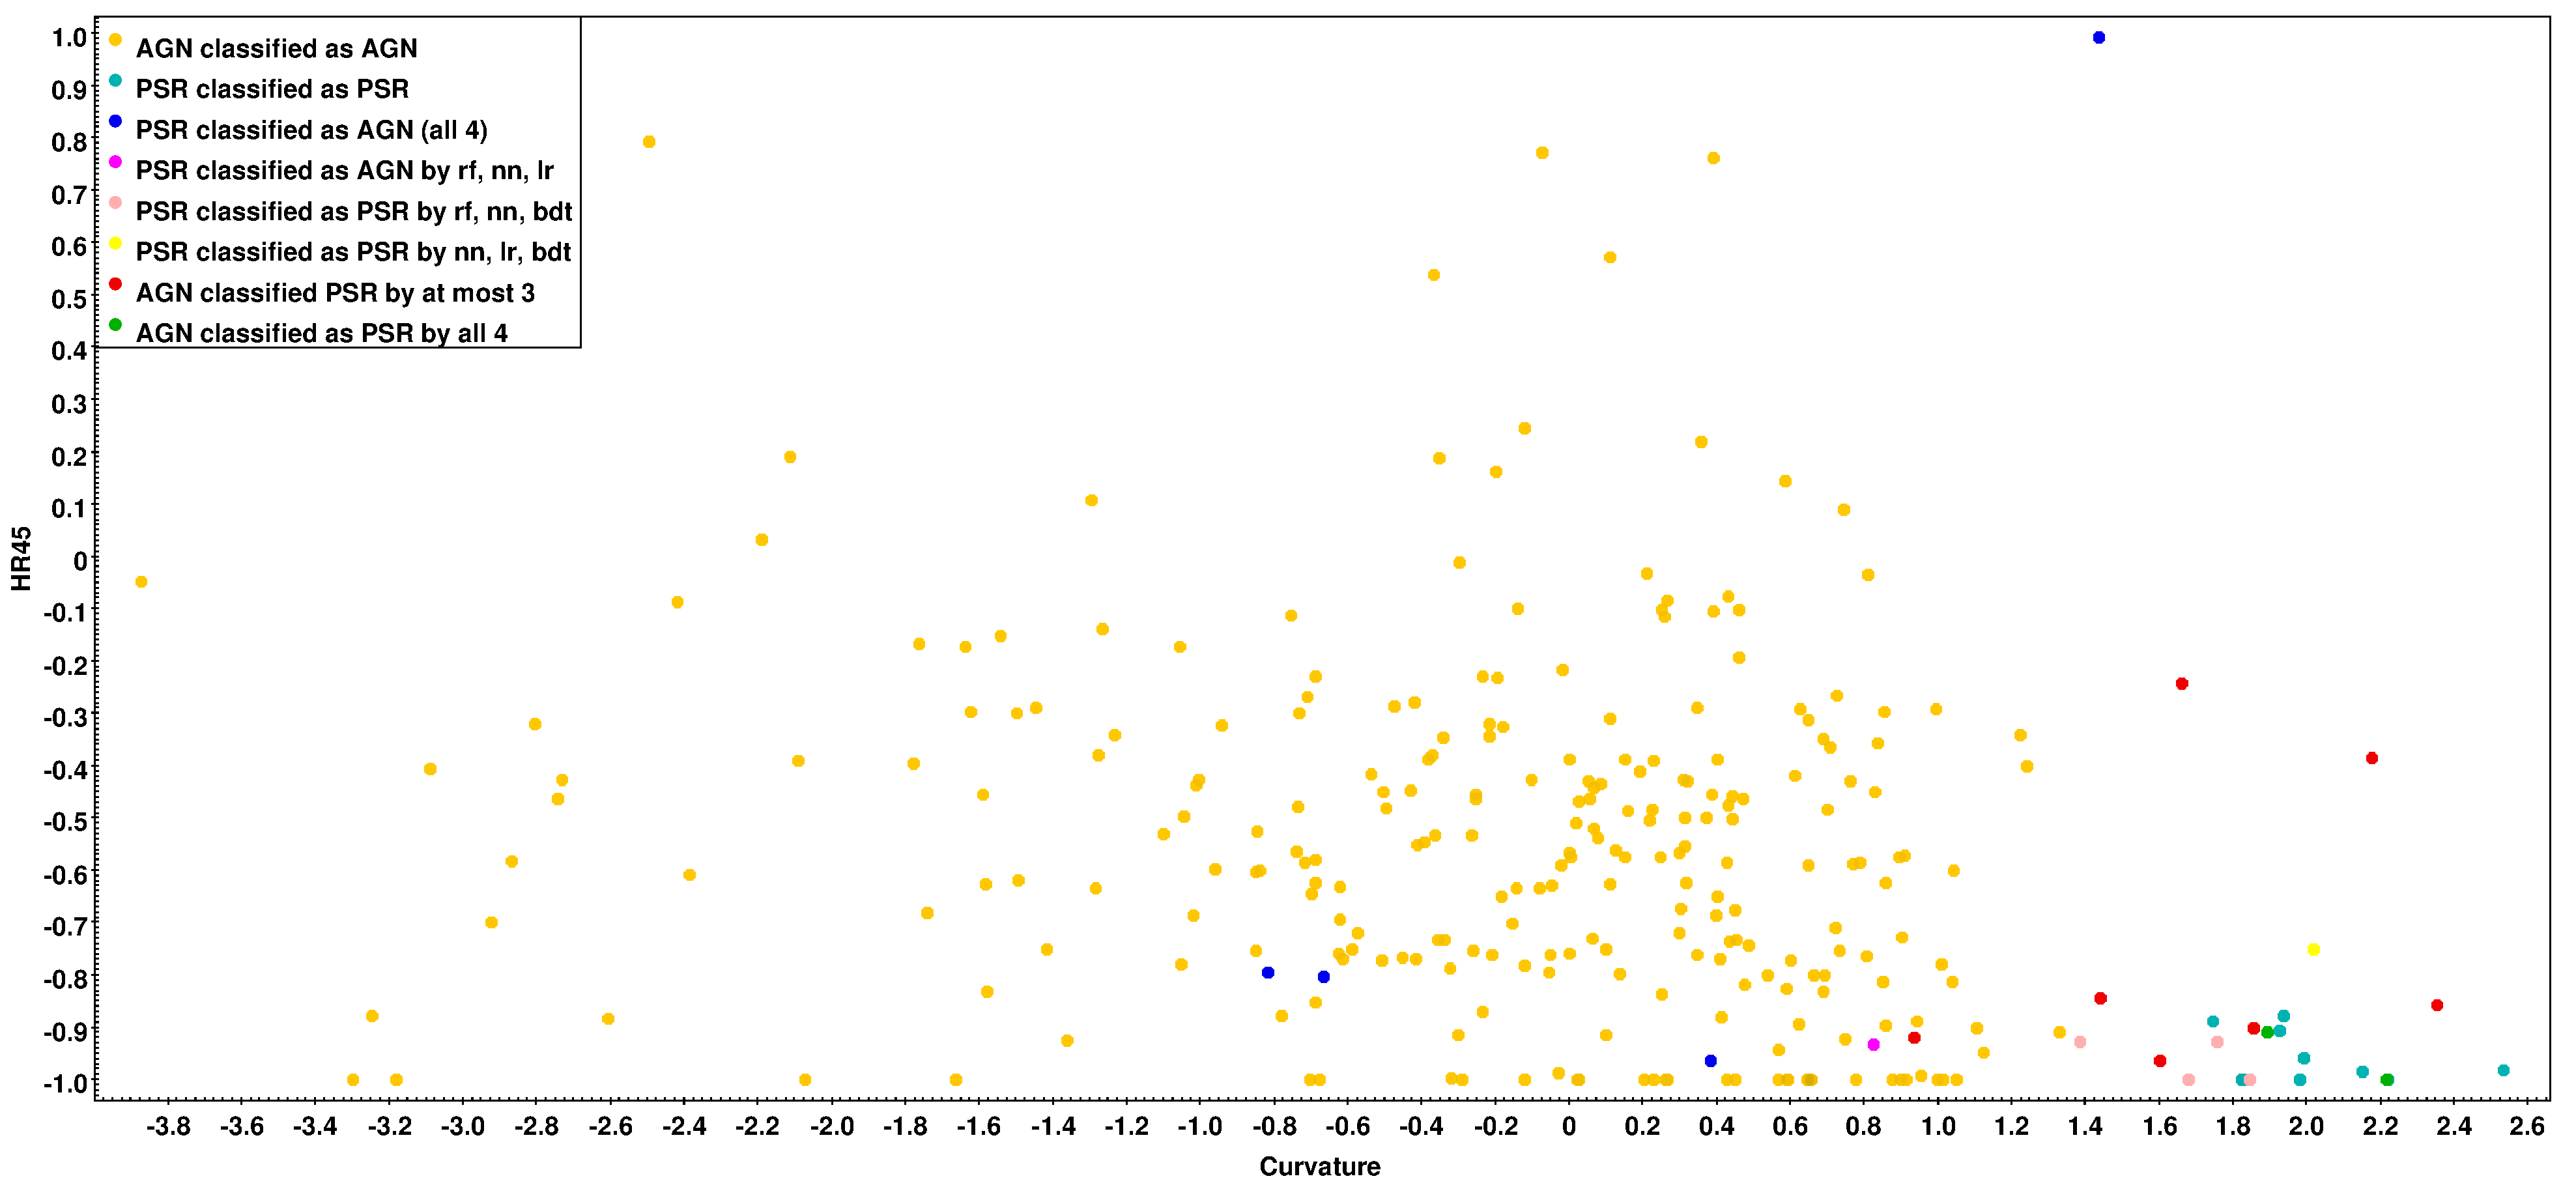
\includegraphics[width=\twopicsp\textwidth]{plots/final_catalog.pdf}
\label{fig:corr_mat}
\end{figure*}
\end{comment}

For the classification of 4FGL sources, we do not perform another optimization of meta-parameters, i.e., we used the same meta-parameters for the four algorithms as in the construction of the probabilistic catalog based on 3FGL, except for NN where we increased the number of neurons in the hidden layer to 16. Similar to the construction of the 3FGL probabilistic catalog, we use both unweighted training samples and oversampling, i.e., we have 8 classification methods.
We retrain the algorithms using the 16 features for the 4FGL sources.
The corresponding accuracies are reported in Table \ref{tab:selected_algs2}.
All algorithms have a slightly better accuracy for the 4FGL-DR2 catalog compared to the 3FGL catalog, which is likely due to a better determination of the spectra in 4FGL, to a higher number of features, and more associated sources used as training data. 

% (same as the number of features). However, due to the number of features being higher, we hypothesized that the Neural Network should under-perform as compared to before.

\begin{table}[!h]
\resizebox{0.45\textwidth}{!}{
    \tiny
 %  \centering
    \renewcommand{\tabcolsep}{0.4mm}
\renewcommand{\arraystretch}{1.6}

    \begin{tabular}{|c|c|c|c|}
    \hline
    Algorithm&Parameters & Testing Accuracy & Std. Dev.\\
    \hline
    RF& 50 trees, max depth 6  &97.87 & 0.36\\
    RF\_O   &&97.56&0.39 \\
    \hline
    NN & 300, 16 Neurons, Adam & 97.41 & 0.47\\
    NN\_O&&95.48&0.66\\
    \hline %\midrule   -> aakash do you mean this?
    BDT & 100 trees, max depth 2    &   97.63 &0.39\\
    BDT\_O&&97.72&0.38\\
%    \hline %\midrule   -> aakash do you mean this?
%    BDT & 200 trees, max depth 2    &   95.8  \\
    \hline
    LR & LBFGS solver, 200 iterations & 97.80&0.38\\
    LR\_O&&96.03&0.53\\
    \hline
     
    \end{tabular}}
    \vspace{0.2cm}
    \caption{Testing accuracy of the 4 algorithms on 4FGL-DR2 associated data. ``\_O'' denotes training with oversampling.}
    \label{tab:selected_algs2}
\end{table}

The expected numbers of pulsars and AGNs among the 1658 unassociated sources in 4FGL-DR2 without missing values are
presented in Table \ref{tab:4FGL-DR2}.
The definition of columns and rows is the same as in the 3FGL catalog case in Section \ref{sec:3FGLprediction1}.


\begin{table}[!h]
\resizebox{0.45\textwidth}{!}{
    \tiny
 %  \centering
    \renewcommand{\tabcolsep}{0.3mm}
\renewcommand{\arraystretch}{1.5}

    \begin{tabular}{| l |c|c|c|}
    \hline
    Correction for other sources & AGNs & Pulsars & Mixed \\
    \hline
    Uncorrected &  872 & 162  &  624 \\
    \hline
    Corrected & 820.8  & 134.6  & 563.2 \\
    \hline
     
    \end{tabular}}
    \vspace{0.2cm}
    \caption{Expected numbers of pulsars and AGNs among unassociated sources in the 4FGL-DR2 catalog \citep{2020arXiv200511208B}.
    For definitions see Table \ref{tab:3FGL_prediction}.}
    \label{tab:4FGL-DR2}
\end{table}


Finally, we looked at sources which were unassociated in both 3FGL and 4FGL (using 'ASSOC\_FGL' as an identifier for 3FGL sources). Out of 302 such sources, 38 sources are predicted to be pulsars using 3FGL features and 75 sources are predicted to be pulsars using 4FGL features. This leads to 29 sources which are predicted by all eight methods to be pulsars for features taken from both 3FGL and 4FGL catalogs. Among these 29 sources, four can be spatially associated to pulsars in the Parkes survey (of the other two, one is now associated as a pulsar in 4FGL, and the second one is not detected in 4FGL).  For convenience, we save these 29 pulsar candidates as a separate file.



